\section{The Design Space of Tubes}

We propose the use of tubes to redirect active components through the core and onto the surface of 3D printed interactive objects.  By using different types and topologies of tubes and inserting different media into the completed tubes, a variety of input and output types \valkyrie{need clearer word than ``types"} can be located at arbitrary points on the surface of a 3D print.  We describe the design space of tubes, and then follow up with some of the input and output possibilities---both those that have been previously explored and those that are possible but remain unexplored.

\begin{figure}[h]
\centering
    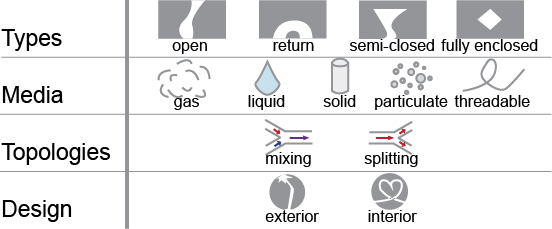
\includegraphics[width=3.4in]{figures/tubespace.png}
\caption{The design space of tubes.  Tube types, media, topologies, and design are discussed more fully in the text.}
\label{fig:tubespace}
\end{figure}

\subsection{Types of Tubes}

Tubes can come in four types: open, return, semi-closed, and fully enclosed.  Each of these types offers distinct interaction capabilities (see Figure \ref{fig:tubespace}).

Open tubes originate from the system side and connect the user side, with both ends of the tube open.  This type of tube may be used to create, for example, capacitive sensors: an open tube filled with conductive paint can be connected to a sensing platform (e.g., Arduino) on the system side, while a user can touch the uncapped other end of the tube.  Using Swept Frequency Capacitive Sensing \cite{Sato-touche} or other techniques, a user's touch of the open end can be sensed.  An open tube can also be used for output, for example by creating in-air vortices as in \cite{Sodhi-aireal}.

A return tube originates at the system and returns back to it.  By threading an electroluminescent (EL) wire through a clear return tube, a maker can create a custom piece of neon art.  If a return tube passes very close to the surface of a 3D printed model, warm or cold water passed through the tube could be used for temperature-based haptic feedback.

Semi-closed tubes are open at the system end (for control of the enclosed medium) and closed at the user end.  We believe this closed interface is most interesting when it is fabricated from a mobile material: for example, a series of tubes terminated in thin rubber membranes on the user side can be actuated by an air pump to create haptic feedback.  Without a printer capable of fabricating flexible material, a maker could affix a balloon to an open tube's end to behave similarly; another possibility is to use semi-closed tubes as audio-generating resonance chambers.

While possible to create, a tube which is open on the user side and closed on the system side is outside our focus on computer-mediated interaction, and we therefore do not discuss these tubes.

A fully enclosed tube has no openings on either the system side or the user side.  Fully enclosed tubes can be used as resonance chambers (e.g., for object identification), or as air bubbles (e.g., as used in \cite{Willis-printedoptics} for internal display).  Their physical design space is very limited, as any support material required to create their internal geometry cannot be accessed for removal.

\subsection{Media in Tubes}

Tubes can be filled with a variety of media to create different interface affordances and capabilities.

``Gas'' comprises all compressible fluids.  Use of fluid pressure inside tubes can create haptic feedback at semi-closed interfaces, or the gases can be used as carriers for scents or fog.  As in \cite{Slyper-pressure}, structures can be engineered to change in air pressure when manipulated correctly (e.g., a spiral that changes pressure when twisted, but not pressed), and thus fluid pressure can also be used as an input.

Incompressible fluids (``liquids'') can perform many of the same interface tasks as gases.  One opportunity with liquids is to fill the interior of tubes with them and cap the ends.  In addition, one can use driable conductive fluids, such as copper paint, to coat the interior of tubes and allow them to function as arbitrarily-shaped wires.  This is especially helpful for the creation of a shared ground, or for creating single-wire capacitive interfaces amenable to sensing with SFCS \cite{Sato-touche}.

Tubes need not have hollow centers: in the case where routed tubes are filled with solid material---in particular, a solid material different from the model material---, interactions such as those in \cite{Willis-printedoptics} are possible.

Particulates, either printed in-place or inserted, can be of varying densities.  A single particle can be used for display.  Sparse particles in a stream of fluid can provide haptic feedback.  Dense particles in a semi-closed tube allow for jamming-based interactions at any point on the surface of an object \cite{Follmer-jamming}.

Threadable inserted elements, such as electroluminescent (EL) wire or fiberoptic cables, are those that can be threaded through tubes post-printing.  This allows overcoming limitations of printers: for example, a Printed Optics-style interface can be created on an inexpensive consumer-grade 3D printer using tubes and inserted fiber optic cable.

\subsection{Topological variations}

Tube topology enables different types of interactions.

Splitting or mixing tubes offer flexibility in output.  If a maker wished to create a painting device, she might wish to have two system-side tubes feeding in primary-colored red and blue paints which mix in varying ratios, allowing their pigments to combine before purple exits from the device (see Figure \ref{fig:tubespace}).  Splitting can also be useful, for example if our maker wants red paint output in two locations from her painting device, she could have one system-side tube, but split the tube into two (see Figure \ref{fig:tubespace}).

Star and tree topologies are extensions of the splitting and mixing primitives.  Using a star topology in which the tubes were filled with conductive paint, we created a toy with several touch-sensitive areas, see Figure \ref{fig:toy}.

\subsection{Features of Tubes}

Tubes may emphasize either their exterior features (connection points) or their interior paths.  These two features lead to different kinds of interfaces.  An example interface that focuses on the exterior connection points is the touch sensitive toy in Figure \ref{fig:toy}, where tubes must exit the toy at the eyes, ears, tail, etc.  An interface focused on the internal path of the tube is the neon sign in Figure \ref{fig:neon}: output is based on the shape of the tube.

\subsection{Inputs and Outputs}

\subsection{Interaction Techniques}
These didn't get discussed yet.
\begin{itemize}
\item \cite{Iwata-volflex} - a display made up of many balloons that inflate and deflate to change the shape
\item \cite{Kim-inflatablemouse} - a basic mouse, but it inflates so you can store it and also use it more reasonably than a flat mouse
\item \cite{Hashimoto-squirming} - hold a speaker in your hands, and air pressure changes make it feel like you're holidng a living, squirming thing
\end{itemize}

\valkyrie{this section includes related work.  is that ok?  it's in the table, and I think we should cover the related input techniques here rather than in the designated related work section (which I think is more suited to fabrication and routing stuff).}

By crossing tube types, topologies, and inserted media, we create a space of possible inputs and outputs that can be tube-mediated.  We offer a table (see Figure \ref{fig:designspace}) containing these possibilities, referencing previous work on input/output techniques where appropriate, noting that many of these techniques have not been attempted using digital fabrication.  We suggest new points in the design space that have been unexplored or not yet explored with digital fabrication.

\begin{figure*}[t]
\centering
    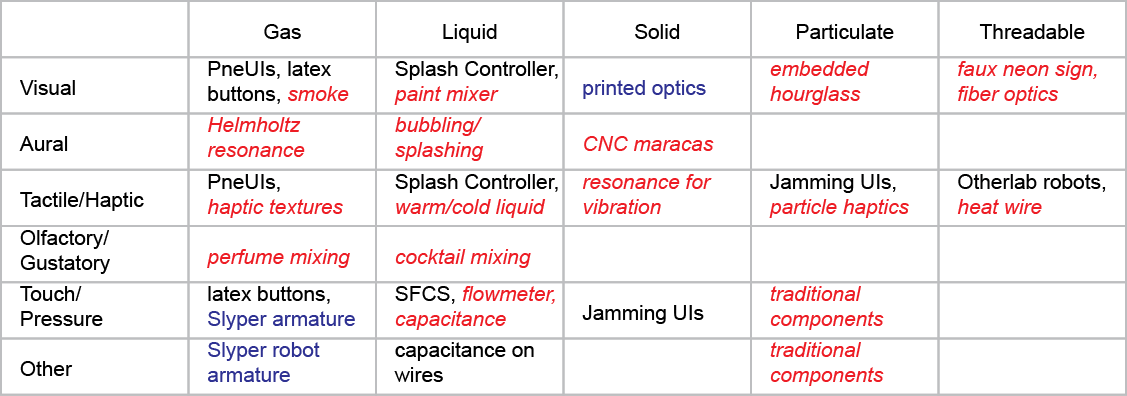
\includegraphics[width=\textwidth]{figures/designspace.png}
\caption{The design space of tube-based interactions.  Existing systems are written in regular font.  Those created with fabrication are in {\color{blue}blue}. In \emph{{\color{red}red italic}} are unexplored interactions creatable with custom-fabricated tubes.  Darker grey is output.  Lighter grey is input.  \valkyrie{I don't know what else might go in the blank spaces... looking for suggestions!  Also, I'm not confident this breakdown is the most clear: for example, the "liquids" category includes the copper paint, which functions as wires ("threadables"), but takes the form of a liquid...  and the general presentation of the table could probably be better in some way.}}
\label{fig:designspace}
\end{figure*}

\subsubsection{Inputs}

Tubes create opportunities for many types of input sensing across the surface of printed devices.  We describe sensing touch, pressure, grasp, flexing, tapping, and manipulation of traditional electronic components.  We recognize that there are likely more input sensing techniques, both existing and on the horizon, that are compatible with the use of tubes.

Touch sensing is enabled through tubes filled with conductive media.  Traditional wires (threadable) may be used, but we have had success with conductive paint (liquid).  Using conductive paint and Swept Frequency Capacitve Sensing (SFCS \cite{Sato-touche}), an interior star tube topology can enable single-wire touch- and grasp-sensing at any set of points on a printed object's surface (see Figure \cite{fig:toy}).  Simple capacitance measurements are possible using the same media, and custom-designed sensors like those created in Savage, et al.,'s Midas system are also possible \cite{Savage-midas}.

Pressure can be sensed in multiple ways.  Slyper, et al., in \cite{Slyper-pressure} contribute a set of semi-closed fabricatable primitives that respond to particular actions, like twisting or pushing, with changes in internal air pressure.  \valkyrie{that sentence is not clear}  These primitives can be attached at the terminus of any semi-closed tube; the user can manipulate the printed endpoint and the system can sense air pressure changes.  Pressure can also be more simply sensed via capacitance using those techniques.

Grasp sensing can also be enabled using Wimmer's FlyEye technique \cite{Wimmer-flyeye}.  This technique involves a pair of optical links at each point of interest: one of each pair is connected to an infrared (IR) LED and the other to a camera.  When some object nears or touches a pair of cables, IR light from the LED is reflected back to the camera and the touched point appears as a bright spot.  Follmer, et al.,'s Jamming User Interfaces \cite{Follmer-jamming} rely dense particulates enclosed in a flexible volume, and can be sensed optically.  These dense particulates can be printed in-place with desired characteristics (such as varying particle size or shape) using sacrificial support material, or added post-print.  The optical links necessary for sensing with FlyEye or Jamming can be created either via clear solid cores as in \cite{Willis-printedoptics} or via fiber optic cables threaded through hollow tubes (see Figure \ref{fig:pens}).

Some 3D printers, like our Objet Connex 260, can fabricate rubber-like materials.  Much like Slyper, et al., in \cite{Slyper-shape}, we can sense flexing and bending of prints made on these machines.  While Slyper, et al., created multi-level multi-stage silicone molds with embedded wires to build their sensors, by placing tubes in our rubberlike prints and inserting conductive media afterwards, we can perform the same flex sensing.

Tapping is another input possibility.  Due to differential sound conductivity in different printed materials (in particular, the rubberlike Objet material compared to the hard Objet material \valkyrie{presumably we should get or take some measurements of this and include it in the appendix?}), tubes of a greater conducting material can be embedded in a model of a lesser conducting material.  A microphone or piezo placed at the system-side of these sound-conducting tubes can determine where the model was tapped and how it was tapped.  Active acoustic sensing as described in Touch \& Activate \cite{Ono-touchandactivate} is also possible; this technique would allow for particular areas of interest (connected to sound-conducting tubes) to be touch sensitive, while other areas (made of non-conducting material) are not sensed.

Sensing via traditional electronic components (e.g., potentiometers, alcohol gas sensors) can be accomplished by conductive inserted media.  Components can be recessed into a print's surface, with their leads implanted into open tubes.  By inserting liquid copper paint instead of threading traditional wires, all components in a model can share a ground line, and the paint's drying process obviates the use of solder or glue to affix the components in place (see Figure \ref{fig:embeddedcomponents}).

\begin{figure}[h]
\centering
    
\includegraphics[width=3.4in]{figures/series-of-tubes.jpg}
\caption{This sphere has a recessed space to hold a potentiometer.  The potentiometer and the LEDs share a ground, seen by the translucent rendered view in (b).}
\label{fig:embeddedcomponents}
\end{figure}

\subsubsection{Outputs}

While many input techniques require the use of conductive media inserted into tubes, output media are more varied.  We describe potential tube-based outputs organized by the five senses: visual, aural, haptic, and olfactory/gustatory.  In addition to outputs we mention explicitly, any outputs possible using traditional electronic components are possible as described above.

\emph{Visual} outputs can be mediated by gases, liquids, solid, particulates, or threadables.  EL wire can be threaded through custom paths to create neon signs, as in Figure \ref{fig:neon}.  Colored liquids can be mixed and split before exiting an opaque device, or in a transparent device their mixing, splitting, and paths could be used for dispaly.  PneUIs \cite{Yao-pneui} can be fabricated as single parts: the rubberlike material offered by our Objet is inflatable when thin (200\% elongation at break), and a PneUI located at the terminus of a tube could be actuated by a system-side air pump (see Figure \ref{fig:braille}).  Mechanical motion can be mediated through fluids (a light object which is partially contained in a tube or located at its end could be pushed by the fluid pressure of the tube) or threadables (e.g., muscle wire).  Large particles trapped in tubes visible to the user can be used for, e.g., maze games (see Figure \ref{fig:maze}).  Using techniques like those described by Harrison, et al., in \cite{Harrison-buttons}  \valkyrie{this paragraph seems terrible.  I think all these paragraphs might seem terrible...}

\emph{Aural} outputs can be created with gases.  Zoran has successfully 3D printed a functional flute, which in essence is a long open open tube with semi-closed tubes coverable by keys \cite{Zoran-flute}.  Helmholz resonance (the phenomenon that creates noise when you blow into the top of a glass bottle, which is also how some musical instruments, like ocarinas, work) can be leveraged to create computer-controllable sound chambers.  All that is necessary for this is an enclosed chamber with a tube connected to it via a narrow neck-point (see Figure \ref{fig:ocarina}).  Passive sound amplification (like a phonograph horn) and sound redirection are also possible using tubes.

\begin{figure}[h]
\centering
    
\includegraphics[width=3.4in]{figures/series-of-tubes.jpg}
\caption{This box (a) contains an enclosed Helmholz resonator, seen in the cutaway view (b).  This resonator creates a sound when air is blown through the tube at the top, because air compresses at the small neck joint between the chamber and the tube.  \valkyrie{need to get a test print of this that actually works}}
\label{fig:embeddedcomponents}
\end{figure}

\emph{Haptic} outputs are possible through compressible and incompressible fluids.  Fluids can actuate particulates and create programmable pliability (as discussed above and in \cite{Follmer-jamming}).  Additionally, use of semi-closed tubes with rubberlike material as the caps allows for gases to actuate surface features (see Figure \ref{fig:braille}).  Sodhi, et al., in \cite{Sodhi-aireal} created free-air haptic feedback using controlled vortex generation: this technique could also be reproduced using a series of tubes.

\emph{Olfactory} and \emph{gustatory} outputs can be created through the mixing and splitting of tubes carrying scented or flavored fluids, respectively.

\subsection{Identity}

Tubes included in printed objects allow for their identification.  While the tubes need not be visible (especially in the case of fully-enclosed tubes), their presence, location, and length change the acoustic resonance properties of a printed object.

Both identification by recall and intentional encoding are possible.  As seen in \cite{Ono-touchandactivate}, different objects have different acoustic signatures.  Additionally, two objects that are visually identical but which have fully enclosed (or other types) of tubes on their interior can be distinguised acoustically.  Thus we can recall an object's identity once its acoustic signature has been recorded.

We have also experimented with intentional encoding.  Semi-closed tubes can function as resonance chambers: the first resonant frequency $F_1$ Hz of a semi-closed tube length $L$ meters can be found by $F_1 = \frac{c}{4L}$ (where $c$ is the speed of sound).  All odd harmonics (i.e., $3*F_1$, $5*F_1$, $7*F_1$, ...) of this frequency are also resonant frequencies of the tube. \valkyrie{need to provide some guidelines for the number of IDs we can create in this way, and where in the sound spectrum they are.  my sense is that this will depend highly upon the i/o sensitivities of the mic and speaker selected.}

An object's resonant frequency can be measured by attaching a speaker and microphone to it, sweeping frequencies with the speaker, and performing a Fourier transform on the resultant signal from the microphone.  Peaks in the transformed data correspond to stronger returned impulses: the resonant frequencies of the object.

This is similar to work done by Willis, et al., in \cite{Willis-infrastructs}.  While their technique requires access a terahertz imaging tool, audio resonance identity encoding requires only a microphone and a speaker.

\valkyrie{in my experiments so far, it seems that the material printed does conduct sound fairly well, so this is feasible.  I think we should get some equipment and do a small test, though, since I don't know how the resonance will change with the big hunk of plastic around the semi-open tube.  hopefully discussing this with Alex soon.}